\scanpage{69}
Soit cat. \inserted{$k$-}abélienne $\mathcal M$
\[
\left(\begin{array}{l}
\text{avec }\varprojlim\\
\text{\uline{assez de projectifs $k$-plats}}\\
\text{assez d'injectifs.}
\end{array}\right.
\]
Alors si $f:A\mathbin{\text{---}}B$ est $k$-coasphérique, alors
\[
\unsure{LH^\bullet|LH_\bullet}(B,F)\overset{\simeq}{\mathbin{\text{---}}}LH_\bullet(A,f^*F)
\qquad\forall F\in\widehat B_{\mathcal M}
\]

\deleted{$\operatorname{Hom}(a,$}
\[
\xi\longrightarrow a\otimes_k\xi\qquad\text{transforme mono en mono.}
\]
\margin{$)$}
\[
\xi\mathbin{\text{---}}\operatorname{Hom}(\xi,a)\qquad\text{transforme mono en épi}
\]
\diagram{\begin{tikzcd}
LH_\bullet(A,F)\\
\widehat A_{\mathcal N}\arrow[u]
\end{tikzcd}}
\[
\mathbf{Ab}_k^{\deleted{\unsure{o}}}\qquad
\deleted{\text{\unsure{assez}}}\ \varinjlim
\]
assez de proj

assez d'inj. $k$-co\unsure{plats} ?

OK

\deleted{$\varinjlim$}
\figure{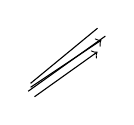
\begin{tikzpicture}
\draw[->](0,0)--(.9,.6);\draw[->](.05,-.12)--(.85,.45);
\draw(0,.05)--(.85,.75);\draw(-.03,-.05)--(.95,.65);
\end{tikzpicture}}
\[
\mathbb Q\qquad\mathbb Q_p/\mathbb Z_p
\]
$\mathrm{Ab}$\hfill$\mathbf{Ab}_k^o$
\[
x\longrightarrow\operatorname{Hom}(x,I)
\]
\diagram{\begin{tikzcd}
B\arrow[r]&\mathrm{Ab}_k\arrow[r]&\mathrm{Ab}_k^o
\end{tikzcd}}
\[
\operatorname{Hom}(J,I)\qquad\text{objet injectif de}
\]
$\mathrm{Ab}_k^o$ i.e. proj.\par
en $\mathrm{Ab}_k$
\mspage{68}
